% Copyright 2004 by Till Tantau <tantau@users.sourceforge.net>.
%
% In principle, this file can be redistributed and/or modified under
% the terms of the GNU Public License, version 2.
%
% However, this file is supposed to be a template to be modified
% for your own needs. For this reason, if you use this file as a
% template and not specifically distribute it as part of a another
% package/program, I grant the extra permission to freely copy and
% modify this file as you see fit and even to delete this copyright
% notice.

\documentclass{beamer}                  % ... or a4paper or a5paper or ...
%\geometry{landscape}                % Activate for for rotated page geometry
\usepackage[parfill]{parskip}    % Activate to begin paragraphs with an empty line rather than an indent
\usepackage{tikz}
\usepackage{pgfplots}
\usepackage{graphicx}
\usepackage[font=small,labelfont=bf]{caption} % Required for specifying captions to tables
\usepackage{dirtytalk}
%\usepackage[version=3]{mhchem}
\usepackage{subcaption}
%\usepackage{subfig}
\usepackage{epstopdf}
\usepackage{pgf}
\usepackage{pdfpages}

\usepackage{subcaption}

\usepackage{booktabs}


%\usepackage[sc, osf]{mathpazo} % add possibly `sc` and `osf` options
%\usepackage{eulervm}
\usepackage{textcomp}
\usepackage{url}
\usepackage[english]{babel} 

%\bibliographystyle{vancouver}


\usepackage{float}
\usepackage{siunitx}
\usepackage[justification=centering]{caption}

\usepackage{mathrsfs}
\usepackage{amssymb}
\usepackage{mathtools}
\usepackage{amsmath}
\usepackage{amsthm}

%\titleformat{\section}[block]{\large\scshape\centering}{\thesection.}{1em}{}

%\titleformat{\subsection}[block]{\bfseries}{\thesubsection.}{1em}{}
\usepackage{csquotes}
%\setlength{\abovedisplayskip}{1pt}
%\setlength{\belowdisplayskip}{1pt}
% There are many different themes available for Beamer. A comprehensive
% list with examples is given here:
% http://deic.uab.es/~iblanes/beamer_gallery/index_by_theme.html
% You can uncomment the themes below if you would like to use a different
% one:
%\usetheme{AnnArbor}
%\usetheme{Antibes}
%\usetheme{Bergen}
%\usetheme{Berkeley}
%\usetheme{Berlin}
%\usetheme{Boadilla}
%\usetheme{boxes}
%\usetheme{CambridgeUS}
%\usetheme{Copenhagen}
%\usetheme{Darmstadt}
%\usetheme{default}
%\usetheme{Frankfurt}
%\usetheme{Goettingen}
%\usetheme{Hannover}
%\usetheme{Ilmenau}
%\usetheme{JuanLesPins}
%\usetheme{Luebeck}
\usetheme{Madrid}
%\usetheme{Malmoe}
%\usetheme{Marburg}
%\usetheme{Montpellier}
%\usetheme{PaloAlto}
%\usetheme{Pittsburgh}
%\usetheme{Rochester}
%\usetheme{Singapore}
%\usetheme{Szeged}
%\usetheme{Warsaw}
%\usetheme{metropolis}
%\usecolortheme{orchid}

\title{Non-constructive mathematics and algorithms}

% A subtitle is optional and this may be deleted
%\subtitle{SI1336 Simulering och modellering}

\author{Jonas Conneryd}
% - Give the names in the same order as the appear in the paper.
% - Use the \inst{?} command only if the authors have different
%   affiliation.

%\institute[Universities of Somewhere and Elsewhere] % (optional, but mostly needed)
%{
%  \inst{1}%
%%  University of Somewhere
%  \and
%  \inst{2}%
%  Department of Theoretical Philosophy\\
%  University of Elsewhere}
% - Use the \inst command only if there are several affiliations.
% - Keep it simple, no one is interested in your street address.

\date{2019}
% - Either use conference name or its abbreviation.
% - Not really informative to the audience, more for people (including
%   yourself) who are reading the slides online

%\subject{Theoretical Computer Science}
% This is only inserted into the PDF information catalog. Can be left
% out.

% If you have a file called "university-logo-filename.xxx", where xxx
% is a graphic format that can be processed by latex or pdflatex,
% resp., then you can add a logo as follows:

\pgfdeclareimage[height=0.5cm]{university-logo}{logo.pdf}
\logo{\pgfuseimage{university-logo}}

% Delete this, if you do not want the table of contents to pop up at
% the beginning of each subsection:
%\AtBeginSubsection[]
%{
%  \begin{frame}<beamer>{Outline}
%    \tableofcontents[currentsection,currentsubsection]
%  \end{frame}
%}

% Let's get started

\pgfplotsset{compat=1.15}
\setbeamertemplate{note page}[plain]
\begin{document}


\begin{frame}
  \titlepage
\end{frame}

%\begin{frame}{Outline}
%  \tableofcontents
  % You might wish to add the option [pausesections]
%\end{frame}

% Section and subsections will appear in the presentation overview
% and table of contents

%%%CONTEXT AND MOTIVATION NY%%%

\begin{frame}{Introduction}
   \begin{itemize}
  \item {Mathematicians have a clear notion of what a proof is.
  } \pause
  \item { (Just don't ask them to \emph{define} what a proof is.)
  } \pause
  \item { Around 1900 there was considerable debate about what constitutes a proof.
  } \pause
  \item { Settled in favor of non-constructive results.
  } \pause
  \item { Constructive mathematics has a spiritual successor in algorithms research.
  } \pause
   \item { Surely, an existence result concerning an algorithm must be the algorithm itself?
  }
  \end{itemize}
\note{

}
\end{frame}

\begin{frame}{The Result That Started It All}
\begin{itemize}
\item Up until the end of the 19:th century, essentially all mathematical results were constructive in nature. 
\pause
\item Although Cantor used some non-constructive results in his theory of sets, the debate around them really started with \emph{Hilbert's Basis Theorem}, proved in 1888. 
\end{itemize}
\pause
\begin{theorem}[Hilbert's Basis Theorem]
If $R$ is a Noetherian ring, then $R[X]$ is a Noetherian ring. 
\end{theorem}
\pause
\begin{itemize}
\item Unimportant what this means. What matters is \emph{how} Hilbert proved it.
\pause
\item One needs to show that a collection of mathematical objects with given properties exists. 
\pause
\item Hilbert did so not by constructing them, but by proving that their non-existence leads to a contradiction.
\end{itemize}
\end{frame}

\begin{frame}{The Objections}
\begin{itemize}
\item A cohort of mathematicians sympathetic towards different constructivist schools were not convinced by this proof. 
\pause
\item Paul Gordan (as in Clebsch-Gordan coefficients) is supposed to have said about this result:

\emph{\say{This is not mathematics; this is theology!}}
\pause

\item Poincaré was another sharp critic. 
\pause
\item The fiercest objector was probably L. E. J. Brouwer (as in Brouwer's fixed point theorem) and sympathisers toward his \emph{intuitionist} school of mathematics. 
\pause
\item There were other constructive schools of mathematics, but we will only have time for intuitionism.
\end{itemize}
\end{frame}

\begin{frame}{What Is Intuitionism?}
\begin{itemize}
\item Let me start by saying that no philosophical position, taken after years of study and contemplation, can be adequately explained in two minutes.
\pause
\item Now, let me explain Brouwer's intuitionism in two minutes.
\pause
\item Hilbert believed in \emph{formalism} - Mathematics is essentially a game about symbol manipulation, with clear, well-defined rules.
\pause
\item In this view, any truth obtained through following the rules of the game should be valid. \pause
\item In contrast, Brouwer thought that mathematics is a subjective activity - the result of constructive mental activity in humans. \pause
\item In particular, a mathematical object is the product of a construction produced by a mind, so its existence is \emph{equivalent} to the possibility of it being constructed.
\end{itemize}
\end{frame}

\begin{frame}{What Is Intuitionism?}
\begin{itemize}
\item Stands in sharp contrast to the usual approach, in which a proof of existence of an object can consist of refuting its non-existence.
\pause
\item Succinctly yet crudely, intuitionists refute the \emph{law of excluded middle} - that for any proposition it holds that either that proposition or its negation are true. 
\pause
\item For this reason, intuitionist mathematicians work without the law of excluded middle.
\end{itemize}
\end{frame}

\begin{frame}{Algorithms and Non-Constructive Results}
   \begin{itemize}
   \item We can all agree, and use all the time, that non-constructive proof methods are valid. 
   \pause
   \item With the advent of computers, constructive mathematics is reborn in the form of algorithms research!
   \pause
   \item In complexity theory, we ask: Can \emph{this} problem be solved \emph{this} efficiently by an algorithm?
   \pause
   \item In complexity theory, efficient $\Leftrightarrow$ worst case running time scales polynomially with the size of the input. Constant factors disregarded. 
   \pause
   \item How does a positive result in complexity theory usually look? A construction of the algorithm.
   \end{itemize}
\end{frame}  

\begin{frame}{Algorithms and Non-Constructive Results}
   \begin{itemize}
   \item How would a non-constructive result in complexity theory look?
   \pause
   \item Proving that there exists an algorithm, without supplying the algorithm?
   
   \end{itemize}
\end{frame}  


\begin{frame}{Introductory Graph Terminology}
\begin{itemize}
    \item To state the results, we need a very short introduction to graphs.
    \pause
    \item A \emph{graph} $G = (V, E)$ is a collection of points $V$ (vertices) and lines $E$ (edges) drawn between them. 

    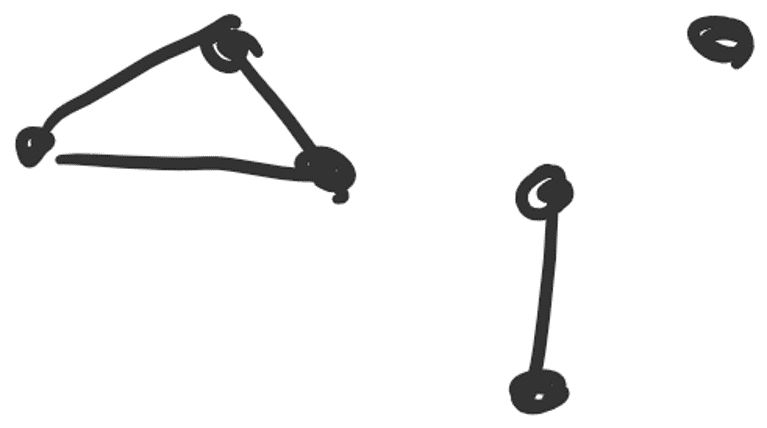
\includegraphics[width=0.2\textwidth]{graf2.png}
    \pause
    \item A graph is not how you draw it; these two graphs are the same graph. 
    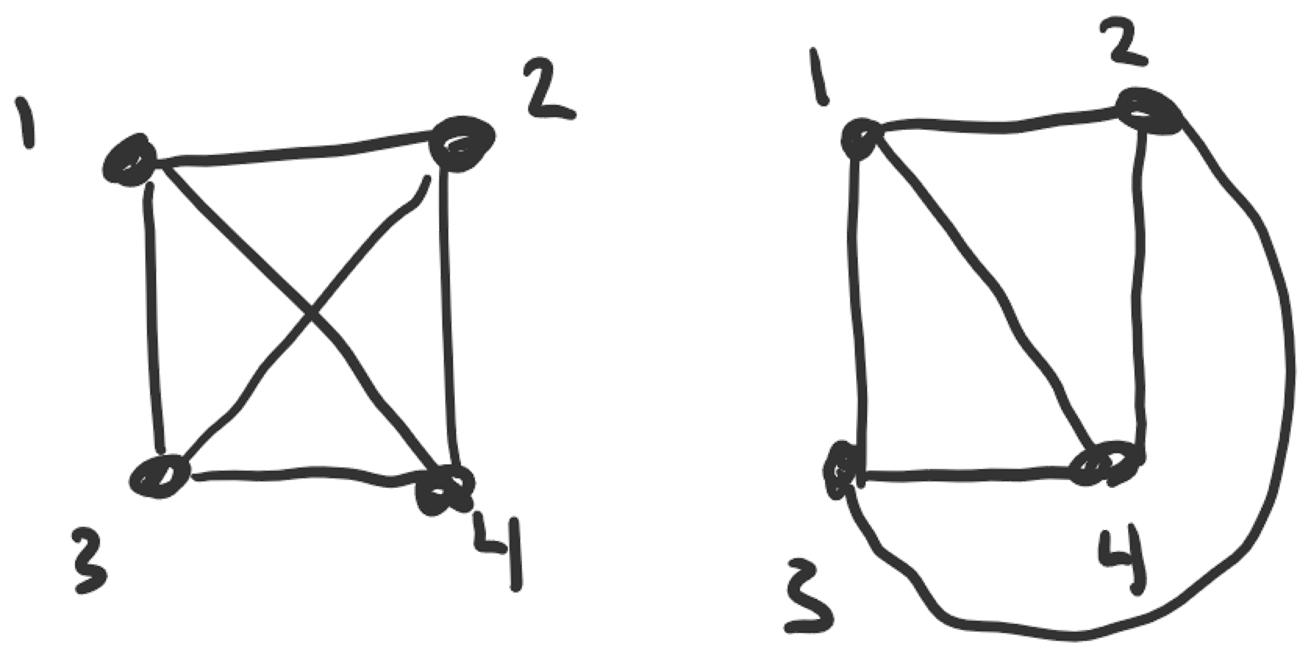
\includegraphics[width=0.3\textwidth]{graf.png}
    \pause
    \item Graphs model pairwise relations between objects and are natural and immensely important in algorithms research.
\end{itemize}
\pause
\end{frame}

\begin{frame}{Introductory Graph Terminology}
\begin{definition}
Let $H$ and $G$ be graphs. $H$ is a \emph{minor} of $G$ if, starting from $G$, we can form $H$ by using only the following operations:
\begin{enumerate}
\pause
    \item Deleting edges. 
    
    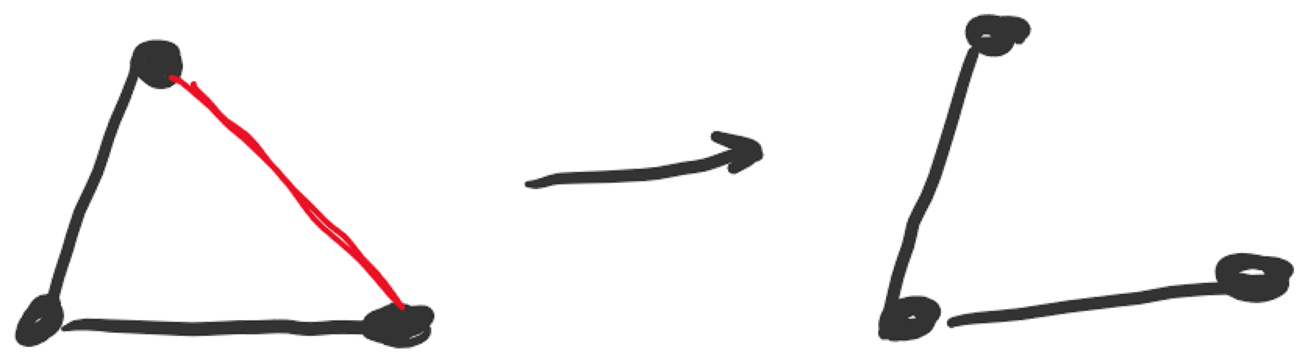
\includegraphics[width=0.3\textwidth]{deleteedge.png}
\pause
    \item Deleting vertices (and also all edges adjacent to that vertex).
    
    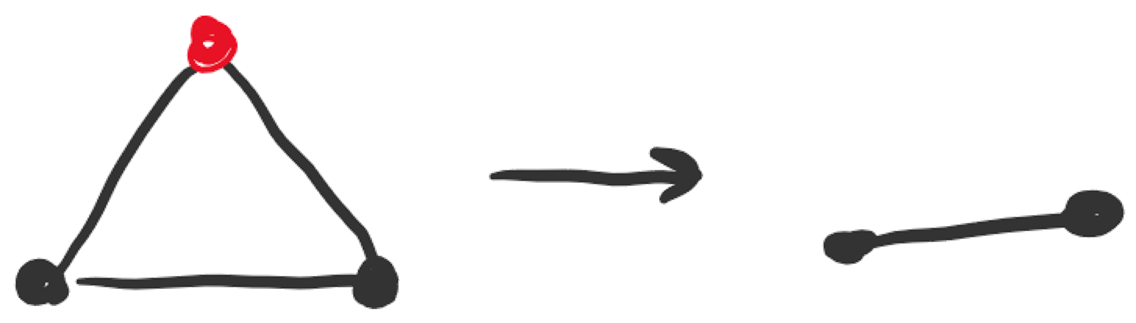
\includegraphics[width=0.3\textwidth]{deletevertex.png}
\pause
    \item Contracting an edge that connects a pair $v_1, v_2$ into a new vertex $v$ which has all neighbors of $v_1$ and $v_2$ as its neighbors.
    
    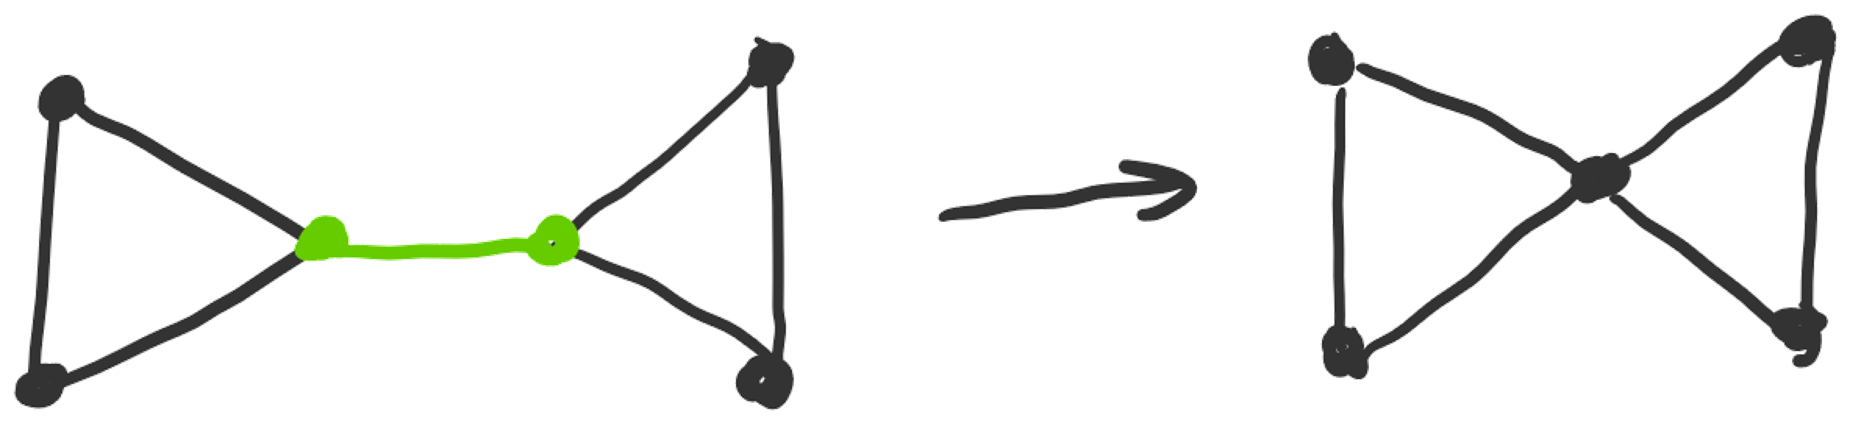
\includegraphics[width=0.4\textwidth]{contractedge.png}
    \pause
    \end{enumerate}
    
    The process of deleting vertices, deleting edges and contracting edges is denoted by \emph{taking minors}.
   
\end{definition}
\end{frame}

\begin{frame}{The Robertson-Seymour Theorem and Related Results}
\begin{itemize}
  \item {
  Naturally, different properties can be defined on graphs. For instance, if a graph can be drawn on the plane without lines intersecting, we say it is \emph{planar}. 
  } \pause
  \item {
  It is not hard to see that a graph retains being planar under taking minors. 
  } \pause
  \item { 
    We can say something very deep about properties that are retained while taking minors.
  }
  \end{itemize}
  \pause
  \begin{theorem}[Robertson-Seymour]
  Suppose a graph property $\mathcal{P}$ is retained while taking minors. Then there is a finite list $L_\mathcal{P}$ of graphs such that a graph $G$ has property $\mathcal{P}$ if and only if none of the graphs in $L_\mathcal{P}$ can be formed from $G$ by taking minors. 
  \end{theorem}
\end{frame}

\begin{frame}{The Robertson-Seymour Theorem and Related Results}
\begin{itemize}
  \item {
  At first glance, it might be hard to see the importance of this theorem.
  } \pause
  \item {
  Regardless, it is an extremely deep theorem with wide-reaching implications, proved during the course of 1983 to 2004 for a total of over 500 pages, by Robertson and Seymour.
  } \pause
  \item { 
  It shows its power related to algorithms when combined with the following result by the same authors:
  }
  \end{itemize}
  \pause
  \begin{theorem}
  Let $H$ be a fixed graph, and let $G = (V, E)$ be an arbitrary graph. Then it can be decided in $O(\lvert V\rvert^3)$ time whether $G$ contains $H$ as a minor.
  \end{theorem}
\end{frame}

\begin{frame}{Algorithmic Implications}
\begin{itemize}
  \item {
  Putting two and two together, we get an extremely powerful algorithmic result:
  } \pause
  \item {
    By the Robertson-Seymour theorem, every graph property $\mathcal{P}$ that is retained while taking minors has a finite list $L_\mathcal{P}$ of graphs such that a graph $G$ has property $\mathcal{P}$ if and only if it contains none of the elements in $L_\mathcal{P}$ as a minor.
  } \pause
  \item{
 We have an efficient (polynomial-time) algorithm to check whether a graph $G$ contains a fixed graph $H$ as a minor. 
  } \pause
    \item{
 Running this algorithm on all the elements in $L_{\mathcal{P}}$ only adds a \emph{constant} factor in the running time.
  } \pause
  \item{
  Therefore, we can decide whether a graph $G$ has \emph{any} given minor-retained property $\mathcal{P}$ in polynomial time in the number of vertices in the input $\Leftrightarrow$ efficiently!
  }
  \end{itemize}
\end{frame}

\begin{frame}{All good! Or?}
   \begin{itemize}
  \item {
  There remains the question of which graphs are in $L_{\mathcal{P}}$ for a given property $\mathcal{P}$. 
   }\pause
  \item { 
  The Robertson-Seymour theorem says nothing about this; it just says that $L_{\mathcal{P}}$ exists and is finite.
  } \pause
  \item {
  It has been proved that no algorithm can find these elements for a given property $\mathcal{P}$. 
  } \pause
  \item {
  We know the elements of $L_{\mathcal{P}}$ for planarity; there are two of them. 
  } \pause
  \item {
  We know that $L_{\mathcal{P}}$, when $\mathcal{P}$ is the property of being able to be drawn on a donut surface without lines intersecting, has at least 17000 elements.
  } \pause
   \item {
  So in general, this is a \emph{non-constructive} result about algorithms!
  }
 
  \end{itemize}
\end{frame}

\begin{frame}{All good! Or?}
\begin{itemize}
 \item {
  As a side note, the algorithm that decides whether a graph $G$ contains a fixed $H$ as a minor has a constant factor that scales superexponentially with the size of $H$. 
  } \pause
  \item {
  If $H$ has 6 vertices, this constant factor exceeds $2^{500,000}$.
  }
  \end{itemize}
\end{frame}

\begin{frame}{Reception}
   \begin{itemize}
  \item {
  No new schools of complexity theory that I know of were formed after this result.
   }\pause
  \item { 
  However, it did call into question whether the characterization of \say{efficient}, and what we accept as a proof in complexity theory are reasonable.
  } \pause
  \item {
  If the purpose of complexity theory is to find efficient algorithms for important problems, what good is a proof like this?
  } \pause
  \item {
  Can an algorithm be called \say{efficient} if it cannot be run in the lifetime of the universe?
  } \pause
  \item {
  One famous computer scientist is supposed to have said about this result:
  
  \emph{\say{This is not computer science; this is a mathematical curiosity!}}
  }
  \end{itemize}
\end{frame}

\begin{frame}{Concluding remarks}
   \begin{itemize}
  \item { 
  Lifting our view, we can note a property that Hilbert's Basis Theorem and the Robertson-Seymour algorithmic result both have: They are very powerful results, proved using innovative techniques.
  } \pause
  \item { 
  Perhaps powerful yet controversial results are precisely what are needed to better understand how we do mathematics. 
  } \pause
  \item {
  For this reason, let us hope the future holds
  more of these strange, wonderful theorems!
  } 
  \end{itemize}
\end{frame}




\begin{frame}{Concluding remarks}
\begin{center}
  \Large{Thank you for your time and your attention!}
\end{center}
\end{frame}

%%%CONTEXT AND MOTIVATION GAMMAL%%%

%\begin{frame}{Context and motivation}
%   \begin{itemize}
%  \item {
%    For systems involving metals, it is desirable to eliminate the explicit treatment of electronic degrees of freedom, since doing so yields significant computational advantages. 
%  } \pause
%  \item {
%    Any effective potential that eliminates explicit treatment of electronic degrees of freedom should be temperature dependent. Temperature dependence in an interparticular potential puts it on a form (non-seperable) such that many properties of conventional integrators, such as symplecticity, may be lost.
%  } \pause
%  \item {
%    Which numerical methods are appropriate for integrating a system in which the interparticular potential is temperature-dependent? The integrator should be symplectic and explicit.
%  } \pause
%  \item {
%    This leads to the investigation of the Tao integration method, which preserves its pleasant properties when integrating non-separable potentials.
%  }
%  \end{itemize}
%\end{frame}

%%%BACKGROUND: HAMILTONIAN SYSTEMS%%%



\end{document}
